%% %% %% %%
%%
%% Parte B de la práctica
%%
%% %% %% %%

\documentclass[../procedimientos.tex]{subfiles}
\graphicspath{{\subfix{../../images/}}}

\begin{document}
\clearpage
\subsection{Parte B}
\subsubsection{Instrucciones}
A partir de las siguientes funciones lógicas, impleméntelas dentro del 
ambiente gráfico de la plataforma \textit{Quatus II} de \textit{Altera}.
\begin{itemize}
  \item $F_1 (xyz) = x (\nt{x} + y\nt{z} + z)$
  \item $F_2 (xyz) = (x + y) (\nt{x} + y) (\nt{y} + \nt{z})$
  \item $F_3 (xyz) = \nt{x}\nt{y} + x\oplus\nt{y}$
  \item $F_4 (xz)  = (x + z)\odot\nt{x}$
\end{itemize}

\subsubsection{Análisis}
De igual forma que en la Parte A, se comenzará haciendo el análsis del 
comportamiento de cada una de las funciones lógicas a través de us tabla de 
verdad. Comenzando con el comportamiento de $f_1(xyz)$.
\begin{table}[H]
  \centering
  \begin{tabular}{ccc|ccc|c}
    \hline
    $x$ & $y$ & $z$ & $\nt{x}$ & $y\nt{z}$ & $\nt{x}+y\nt{z}+z$ & $f_1$\\
    \hline
    0 & 0 & 0 & 1 & 0 & 1 & 0\\
    0 & 0 & 1 & 1 & 0 & 1 & 0\\
    0 & 1 & 0 & 1 & 1 & 1 & 0\\
    0 & 1 & 1 & 1 & 0 & 1 & 0\\
    1 & 0 & 0 & 0 & 0 & 0 & 0\\
    1 & 0 & 1 & 0 & 0 & 1 & 1\\
    1 & 1 & 0 & 0 & 1 & 1 & 1\\
    1 & 1 & 1 & 0 & 0 & 1 & 1\\
    \hline
  \end{tabular}
  \caption{Tabla de verdad de $f_1(xyz)$ (Parte B)}
  \label{tab:b_f1}
\end{table}

Continuando con el comportamiento de $f_2(xyz)$, se tiene que:
\begin{table}[H]
  \centering
  \begin{tabular}{ccc|ccc|c}
    \hline
    $x$ & $y$ & $z$ & $x+y$ & $\nt{x}+y$ & $\nt{y}+\nt{z}$ & $f_2$\\
    \hline
    0 & 0 & 0 & 0 & 1 & 1 & 0\\
    0 & 0 & 1 & 0 & 1 & 1 & 0\\
    0 & 1 & 0 & 1 & 1 & 1 & 1\\
    0 & 1 & 1 & 1 & 1 & 0 & 0\\
    1 & 0 & 0 & 1 & 0 & 1 & 0\\
    1 & 0 & 1 & 1 & 0 & 1 & 0\\
    1 & 1 & 0 & 1 & 1 & 1 & 1\\
    1 & 1 & 1 & 1 & 1 & 0 & 0\\
    \hline
  \end{tabular}
  \caption{Tabla de verdad de $f_2(xyz)$ (Parte B)}
  \label{tab:b_f2}
\end{table}

Se prosigue con el comportamiento de la función lógica $f_3(xyz)$, para esta, 
es primero hacer uso de la equivalencia lógica de la operación XOR, con la 
finalidad de simplificar sus cálculos. Por lo tanto, se obtiene lo siguiente:
\begin{align*}
  f_3(xyz) &= \nt{x}\nt{y} + x\nt{\nt{y}} + \cancel{\nt{x}\nt{y}}\\
  &= \nt{x}\nt{y} + xy
\end{align*}
$$\therefore{f_3(xyz) = \nt{x}\nt{y} + xy}$$

Haciendo uso de la equivalencia anterior, se puede conformar la tabla de 
verdad de la siguiente forma:
\begin{table}[H]
  \centering
  \begin{tabular}{ccc|cc|c}
    \hline
    $x$ & $y$ & $z$ & $\nt{x}\nt{y}$ & $xy$ & $f_3$\\
    \hline
    0 & 0 & 0 & 1 & 0 & 1\\
    0 & 0 & 1 & 1 & 0 & 1\\
    0 & 1 & 0 & 0 & 0 & 0\\
    0 & 1 & 1 & 0 & 0 & 0\\
    1 & 0 & 0 & 0 & 0 & 0\\
    1 & 0 & 1 & 0 & 0 & 0\\
    1 & 1 & 0 & 0 & 1 & 1\\
    1 & 1 & 1 & 0 & 1 & 1\\
    \hline
  \end{tabular}
  \caption{Tabla de verdad de $f_3(xyz)$ (Parte B)}
  \label{tab:b_f3}
\end{table}

Para concluir lo anterior, también se elaborará la tabla de verdad de la 
función $f_4(xy)$, la cual se puede simplificar a través de la equivalencia 
lógica de la compuerta XNOR.
\begin{align*}
  f_4(xz) &= (x + z) \odot \nt{x}\\
  &= \overline{(x+z)}\nt{\nt{x}} + (x+z)x\\
  &= \cancel{(\nt{x}\nt{z})x} + (x+z)\nt{x}\\
  &= (x+z)\nt{x}
\end{align*}
$$f_4(xz) = (x+z)\nt{x}$$

Con la equivalencia anterior se puede elaborar la tabla de verdad, tal como se 
muestra a continuación
\begin{table}[H]
  \centering
  \begin{tabular}{cc|cc|c}
    \hline
    $x$ & $z$ & $\nt{x}$ & $x+z$ & $f_4$\\
    \hline
    0 & 0 & 1 & 0 & 0\\
    0 & 1 & 1 & 1 & 1\\
    1 & 0 & 0 & 1 & 0\\
    1 & 1 & 0 & 1 & 0\\
    \hline
  \end{tabular}
  \caption{Tabla de verdad de $f_4(xz)$ (Parte B)}
  \label{tab:b_f4}
\end{table}

Finalmente, se combinarán los resultados de las Tablas \ref{tab:b_f1}, 
\ref{tab:b_f2}, \ref{tab:b_f3} y \ref{tab:b_f4}, con la finalidad de tener el 
resultado de cada una de ellas en una sola tabla.
\begin{table}[H]
  \centering
  \begin{tabular}{ccc|cccc|c}
    \hline
    $x$ & $y$ & $z$ & $f_1$ & $f_2$ & $f_3$ & $f_4$ & HEX\\
    \hline
    0 & 0 & 0 & 0 & 0 & 1 & 0 & 2\\
    0 & 0 & 1 & 0 & 0 & 1 & 1 & 3\\
    0 & 1 & 0 & 0 & 1 & 0 & 0 & 4\\
    0 & 1 & 1 & 0 & 0 & 0 & 1 & 1\\
    1 & 0 & 0 & 0 & 0 & 0 & 0 & 0\\
    1 & 0 & 1 & 1 & 0 & 0 & 0 & 8\\
    1 & 1 & 0 & 1 & 1 & 1 & 0 & E\\
    1 & 1 & 1 & 1 & 0 & 1 & 0 & A\\
    \hline
  \end{tabular}
  \caption{Resumen del comportamiento de $f_1$, $f_2$, $f_3$ y $f_4$ (Parte 
  B)}
  \label{tab:b_summary}
\end{table}

\subsubsection{Implementación en Quartus}
Para la implementación en la plataforma \textit{Quartus}, se siguió una 
metodología similar a la mostrada en la Sección \ref{subs:a_imp}, con la cual 
se hicieron cuatro archivos de bloques, uno para cada función lógica 
requirida. Los bloques implementados se muestran a continuación.
\begin{figure}[H]
  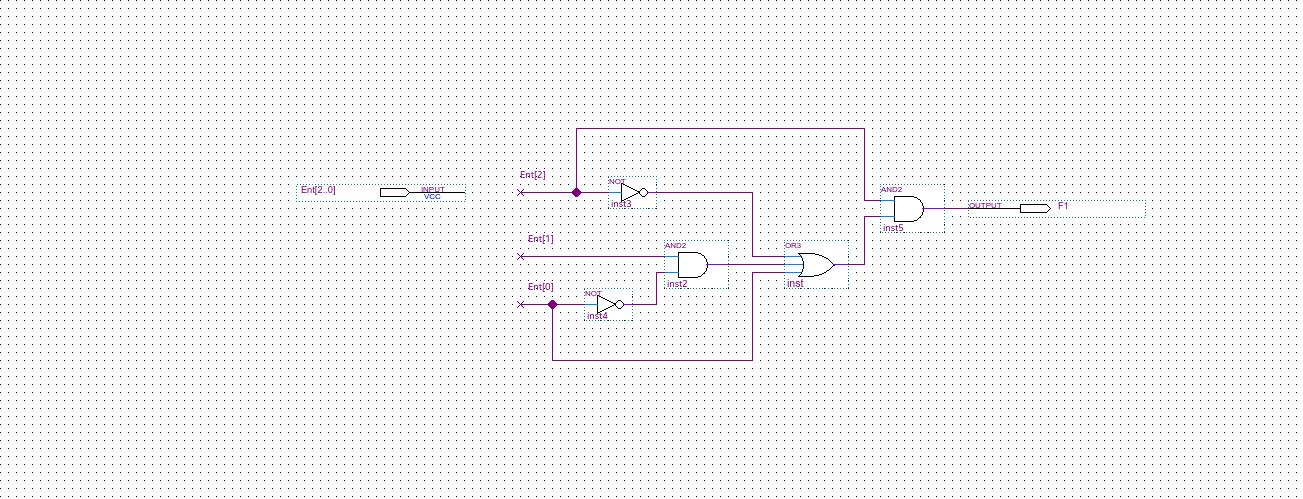
\includegraphics[width=\textwidth]{ejercicio_b1}
  \caption{Implementación de $f_1(xyz)$ (Parte B)}
  \label{fig:b_f1}
\end{figure}
\begin{figure}[H]
  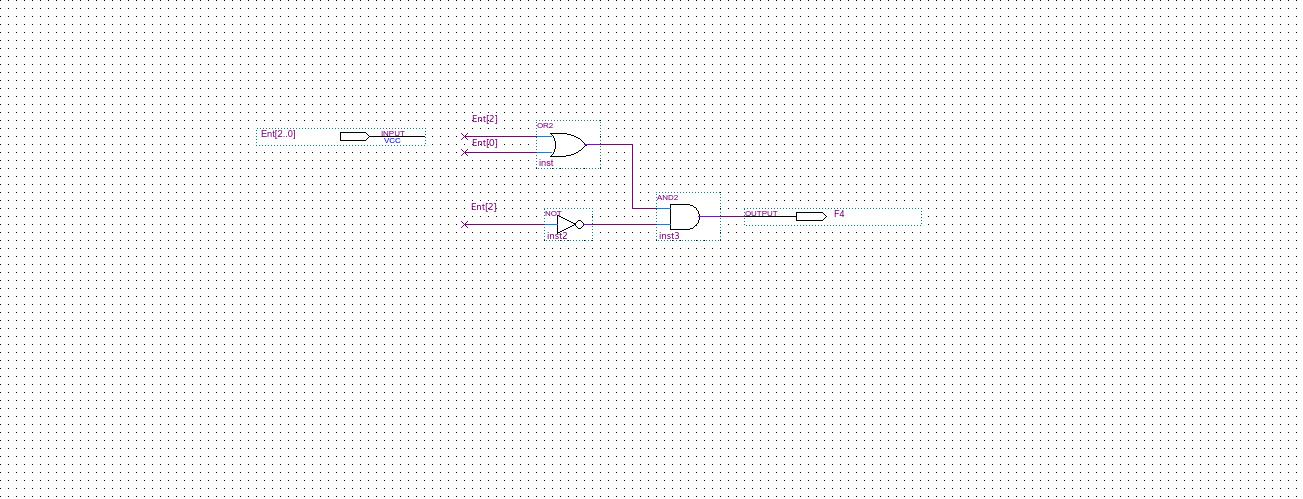
\includegraphics[width=\textwidth]{ejercicio_b2}
  \caption{Implementación de $f_2(xyz)$ (Parte B)}
  \label{fig:b_f2}
\end{figure}
\begin{figure}[H]
  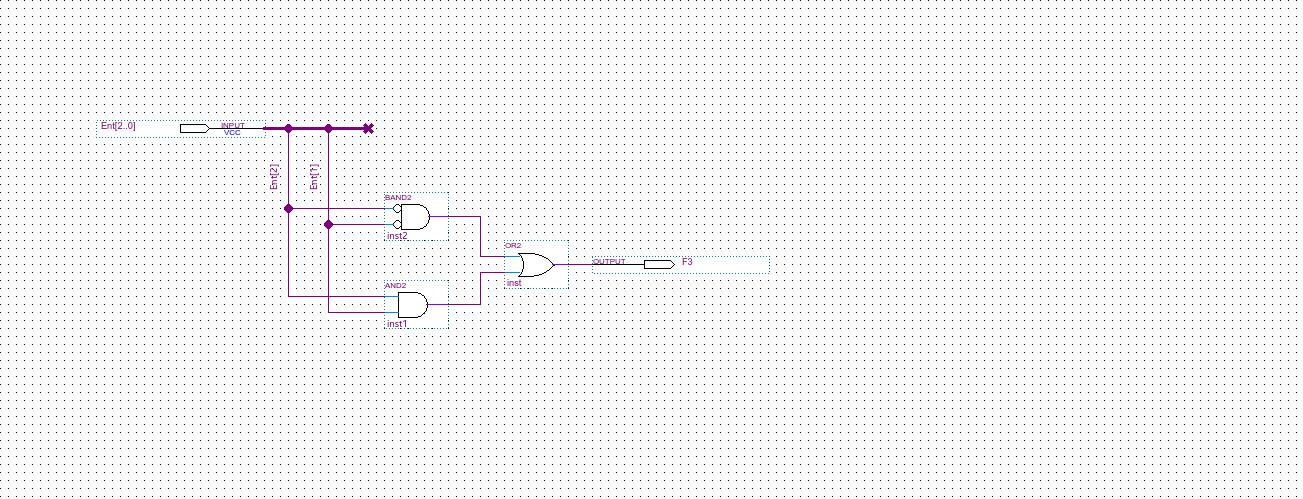
\includegraphics[width=\textwidth]{ejercicio_b3}
  \caption{Implementación de $f_3(xyz)$ (Parte B)}
  \label{fig:b_f3}
\end{figure}
\begin{figure}[H]
  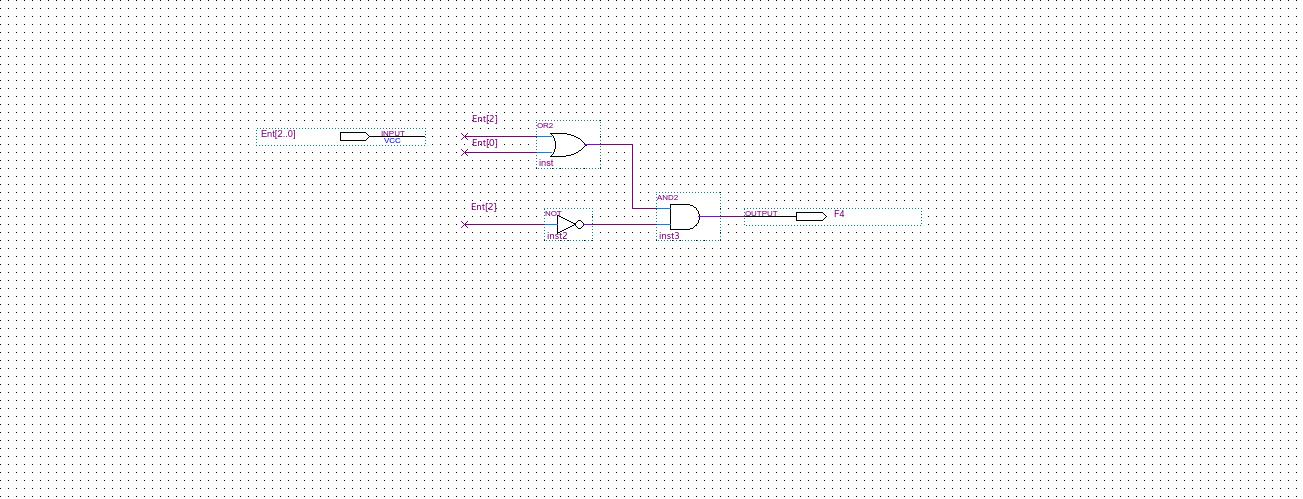
\includegraphics[width=\textwidth]{ejercicio_b4}
  \caption{Implementación de $f_4(xyz)$ (Parte B)}
  \label{fig:b_f4}
\end{figure}

Se hizo uso del concepto de arreglos de señales con la finalidad de 
simplificar la utilización de cada uno de los módulos y así mismo, comprobar 
más sencillamente el funcionamiento de los sistemas. De igual forma, muchas de 
las conexiones se llevaron a cabo a través de la colocación de etiquetas en 
los cables ---tal como aprendimos en la Parte A.

De igual forma, en un archivo de bloques separado fue importante mandar a 
llamar a cada uno de los símbolos previamente creados con la finalidad de 
ponerlos a pruba con un vector de entrada y un vector de salida, tal como se 
muestra a continuación.
\begin{figure}[H]
  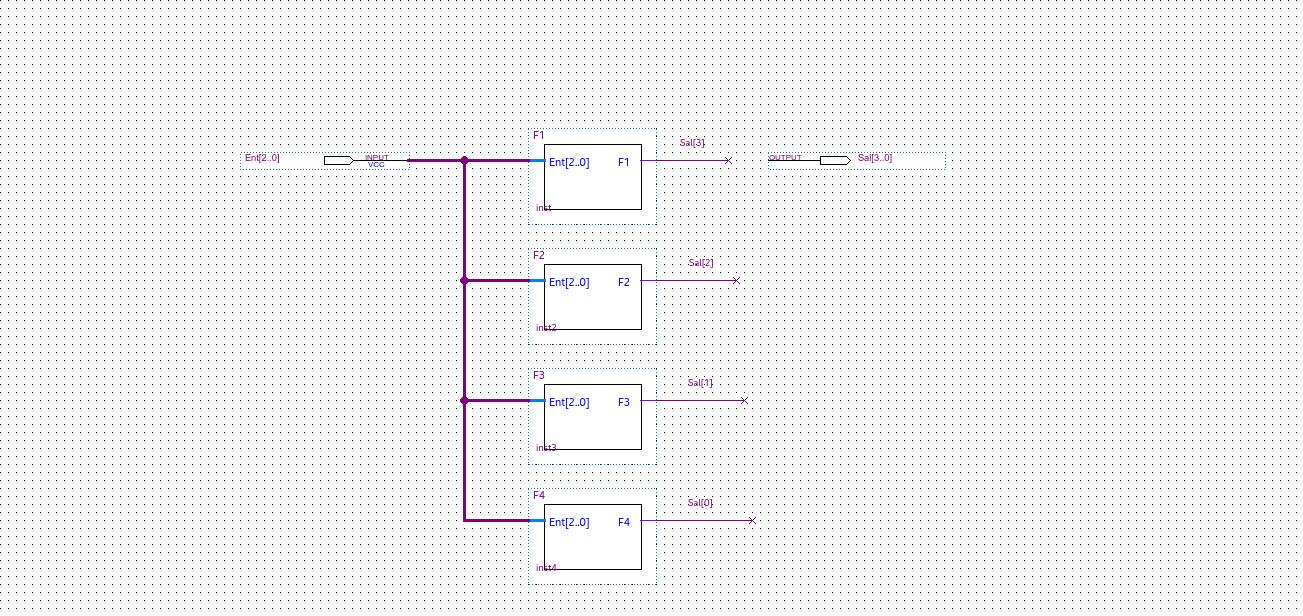
\includegraphics[width=\textwidth]{ejercicio_b}
  \caption{Implementación de la solución (Parte B)}
  \label{fig:b_complete}
\end{figure}

Con lo anterior, fue posible realizar la simulación con ayuda de un archivo de 
tipo \textit{University Program VWF}. Se configuraron las señales a 
visualizar, y se configuraron para tener las entradas mostradas en la Tabla 
\ref{tab:b_summary}. Su utilizó la \textit{Funcional Simuation}, y el resultdo 
fue el siguiente:
\begin{figure}[H]
  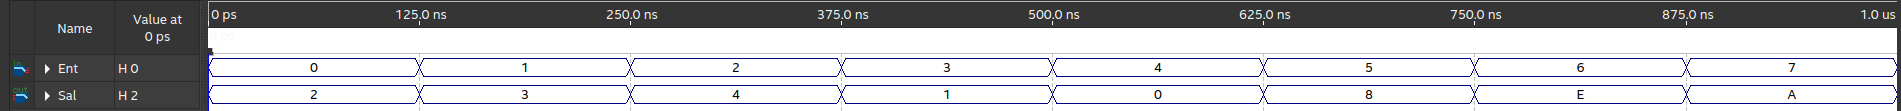
\includegraphics[width=\textwidth]{ejercicio_b_sim}
  \caption{Simulación (Parte B)}
  \label{fig:b_sim}
\end{figure}

Tal como se puede ver en la Figura \ref{fig:b_sim}, los resultados de la 
simulación fueron los mismos que los pre-calculados en la Tabla 
\ref{tab:b_summary}. Los valores del arreglo $Ent$ (codificados en 
hexadecimal) son las señales de entrada; y los valores del arreglo $Sal$ 
(codificados en hexadecimal) son las señales de salida de la función.

\end{document}

